\documentclass{beamer}
%\usetheme{Madrid}
\usepackage{graphicx}
\usepackage{algorithm2e}
\usepackage{multicol}

\title{Hybrid Evolutionary Algorithms for Graph Coloring}
\author{Ernesto Rodriguez\\Vendula Poncova}
\date{\today}
 
\begin{document}
 
\frame{\titlepage}

\begin{frame}
\begin{itemize}
\item P. Galinier and J.K. Hao: \textit{Hybrid evolutionary algorithms for graph coloring}, 1999
\item C. A. Glass and A. Prugel-Bennett : \textit{Genetic Algorithm for Graph Coloring: Exploration
of Galinier and Hao’s Algorithm}, 2003
\end{itemize}
\end{frame}

%%%%%%%%%%%%%%%%%%%%%%%%%%%%%%%%%%%%%%%%%%%%%%%%%%%%%% Problem
\begin{frame}
\frametitle{Graph Coloring Problem}
\centering{
  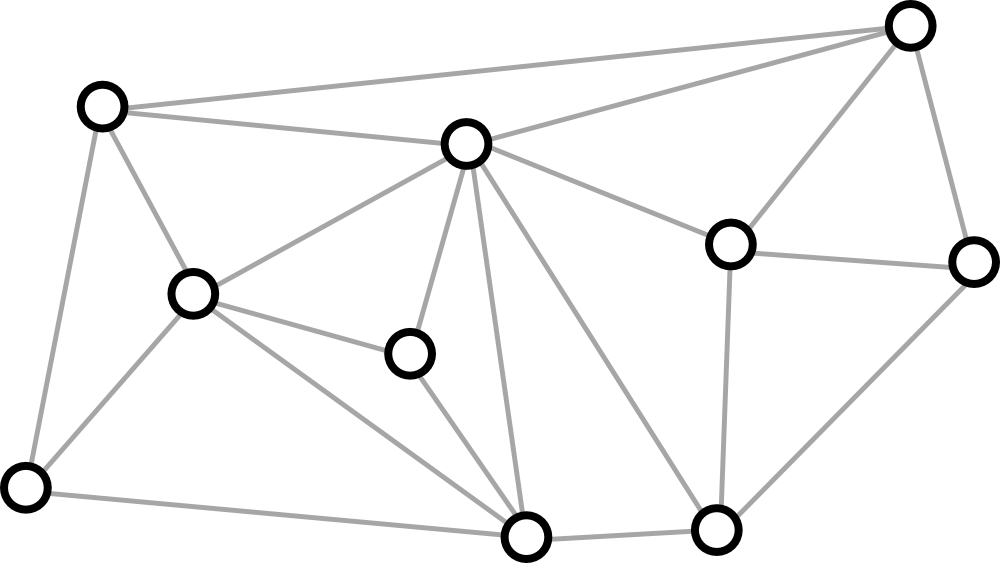
\includegraphics[height=150px]{gc1.png}
}
\begin{itemize}
\item Given a graph $G=(V,E)$, assign a color to each vertex such that no adjacent vertex has the same color
\end{itemize}

\end{frame}

\begin{frame}
\frametitle{Graph Coloring Problem}
\centering{
  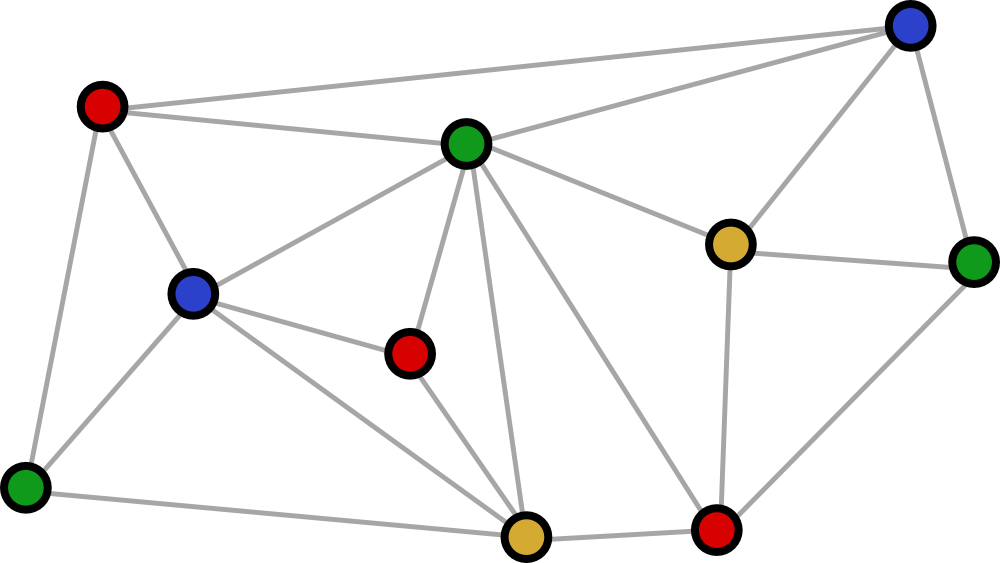
\includegraphics[height=150px]{gc2.png}
}
\begin{itemize}
\item Find the minimum number of colors.
\end{itemize}
\end{frame}

\begin{frame}
\frametitle{Independent set}
\centering{
  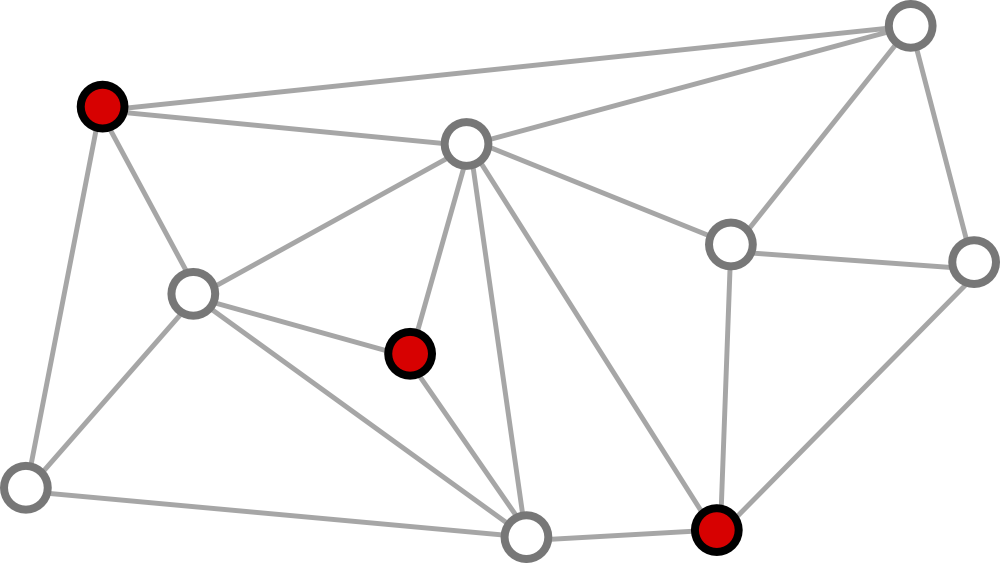
\includegraphics[height=150px]{gc3.png}
}
\begin{itemize}
\item Given an un-directed graph $G=(V,E)$, defined as a set of vertices $V$ and edges $E$, a subset of $V$ is called independent if no two adjacent vertices belong to it.
\end{itemize}
\end{frame}


\begin{frame}
\frametitle{Graph Coloring Problem}
\large{Formally:}
\begin{itemize}
\item A k-coloring is a partition of $G$ into $k$ independent sets
\item An optimal coloring is the smallest k-coloring possible for a graph
\item Want: An optimal coloring
\end{itemize}
\end{frame}

\begin{frame}
\frametitle{Previous Approaches}
\begin{itemize}
\item {\bf Greedy Constructive Methods:} Succesively choose a vertex and a color such that the independent property holds according to some criteria. Poor performance in general.
\item {\bf Genetic Algorithm:} Ordering of vertices encoded as a coloring and use a GA to optimize. No good performance.
\item {\bf Local Search:} Use simulating annealing or tabu search. Differ from each other in the way they define a neighborhood, cost function and search space. State of the art!
\end{itemize}
\end{frame}

%%%%%%%%%%%%%%%%%%%%%%%%%%%%%%%%%%%%%%%%%%%%%%%%%%%%%% Algorithm

\begin{frame}
\frametitle{Hybrid Algorithms}
\begin{multicols}{2}
\begin{itemize}
\item A configuration $s\ \in\ S$ is any partition $s\ =\ \{V_i,..V_k\}$ of $V$ in $k$ subsets
\item A configuration $s$ might not be a proper k-coloring
\item The cost or penalty of a configuration $s$ is the number of conflicting vertices
\item Main difference between a GA: mutation is replaced by a local search operator
\item Early stop if diversity is low
\end{itemize}
\columnbreak
\small{
\begin{algorithm}[H]
\KwData{graph G = (V,E), integer k}
\KwResult{the best configuration found}
{\bf begin}\;
$P\ =\ InitPopulation(|P|)$\;
\While{not Stop-Condition()}{

  $(s1,s2)\ =\ ChooseParents(P)$\;
  $s\ =\ Crossover(s1,s2)$\;
  $s\ =\ LocalSearch(s,L)$\;
  $P\ =\ UpdatePopulation(P,s)$
}
\end{algorithm}
}
where,
\begin{itemize}
\item $L$ is the number of iterations that the local search will perform
\end{itemize}
\end{multicols}
\end{frame}

\begin{frame}
\frametitle{New Crossover Operator}
\begin{itemize}
\item Generic crossover operators perform badly
\item Domain specific knowledge seems to be necesary for this problem
\item {\bf Assignment Approach:} Child inherits the color of a vertex from a parent with equal probability unless it causes a conflict
\item {\bf Partition Approach:} Childs inherit from the parent color classes or subsets of color classes
\end{itemize}

\end{frame}

\begin{frame}
\frametitle{GPX Crossover Operator}
\begin{itemize}
\item Choose a class from a parent which has maximum coloring
\item Remove the vertices of the class from the classes of the parents
\item Assign randomly the vertices left unassigned
\end{itemize}
\end{frame}

\begin{frame}
\frametitle{GPX Crossover Operator}
\centering{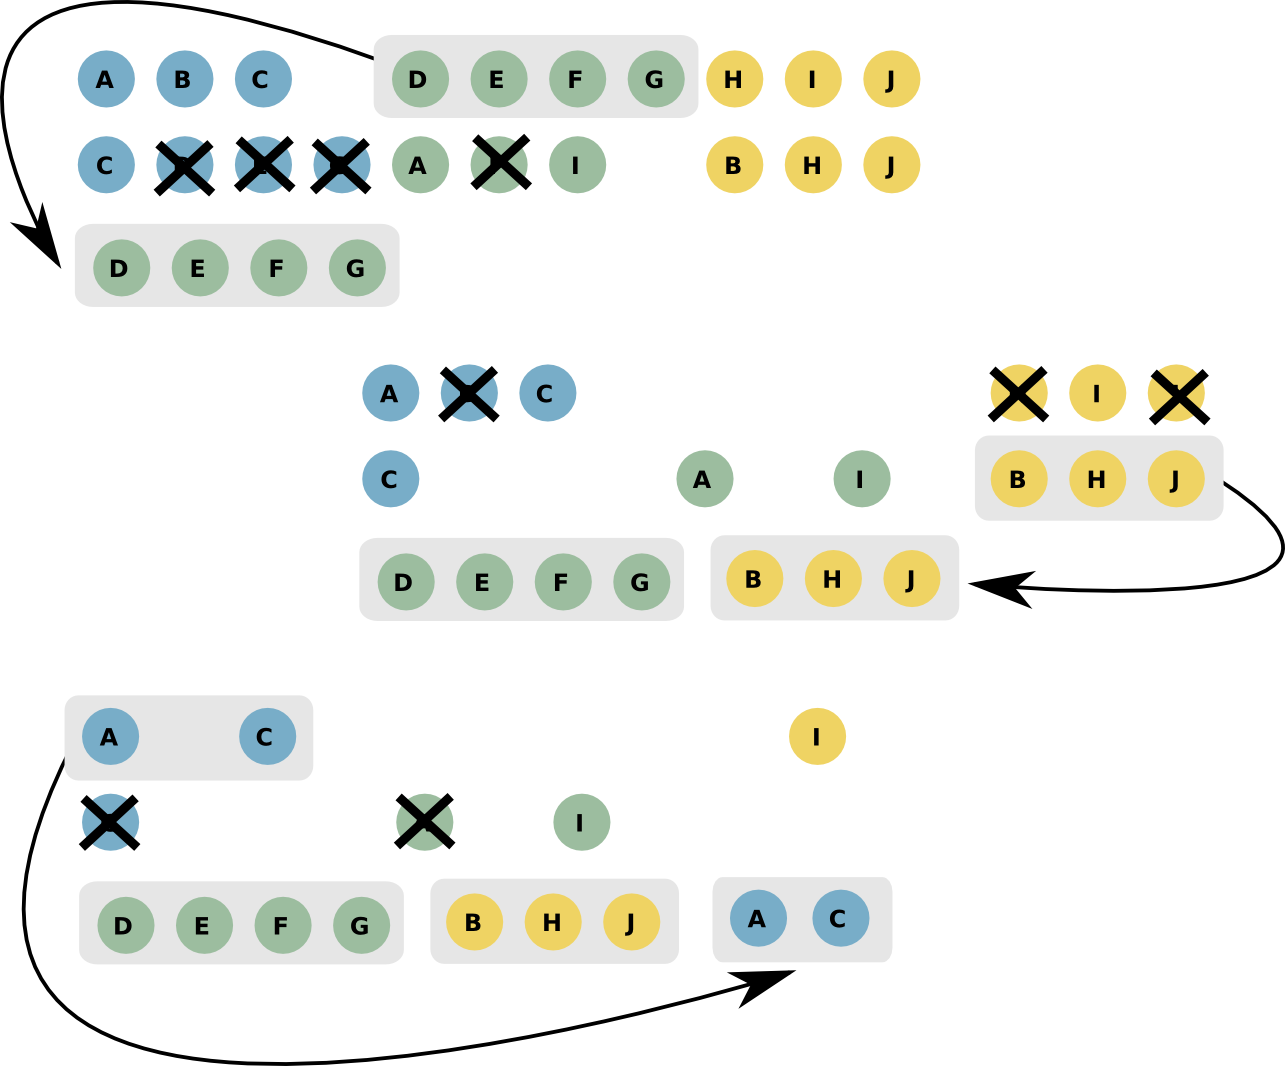
\includegraphics[height=230px]{crossover.png}}
\end{frame}

\begin{frame}
\frametitle{GPX Crossover Pseudo-Code}
\begin{algorithm}[H]
\KwData{configurations $s_1\ =\ \{V_1^1,...,V_k^1\}$ and $s_2\ =\ \{V_1^2,...,V_k^2\}$}
\KwResult{configuration $s\ =\ \{V_1,...,V_k\}$}
{\bf begin}\;
\For{$l\ =\ 1..k$}{

  \eIf{$l$ is odd}{$A\ =\ 1$}{$A\ =\ 2$}
  choose i such tat $V_i^A$ has maximum cardinality\;
  $V_l\ =\ V_i^A$\;
  remove teh vertices of $V_l$ from $s_1$ and $s_2$\;
}
Assign randomly the vertices of $V\ -\ (V_1\ \cup ... \cup\ V_k)$\;
\end{algorithm}
\end{frame}

\begin{frame}

\frametitle{Local Search Operator: Tabu Search}

\begin{itemize}

\item A neighbor is obtained by moving a vertex to another color class
\item A vertex is only moved if it conflicts with other vertex
\item A tabu move which performs better than the best configuration is always accepted
\item The search is repeated for a specific number of iterations $L$

\end{itemize}

\end{frame}

%%%%%%%%%%%%%%%%%%%%%%%%%%%%%%%%%%%%%%%%%%%%%%%%%%%%%% Experiments and results
\begin{frame}
\frametitle{Running Profile}
\centering{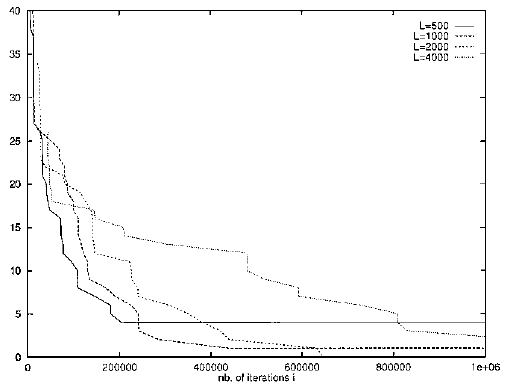
\includegraphics[height=140px]{runProf.png}}
\begin{itemize}
\item {\bf Running Profile:} The best coloring found after a particular number of iterations
\item When $L$ is 500 and 1000, best solution is not found; with 2000 and 4000 best solution is found
\item When $L$ is larger, the search progresses more slowly.
\end{itemize}
\end{frame}

\begin{frame}
\frametitle{Diversity}
\centering{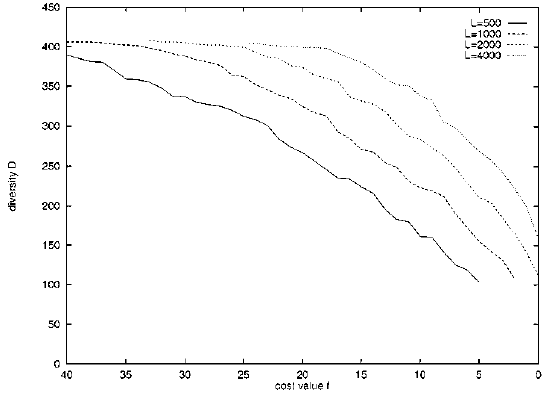
\includegraphics[height=140px]{div.png}}
\begin{itemize}
\item {\bf Difference Function:} Number of transformations to convert one coloring into another 
\item Longer local search sets the children far away from the parents
\end{itemize}
\end{frame}

\begin{frame}
\frametitle{Comparison with Tabu Search}
\centering{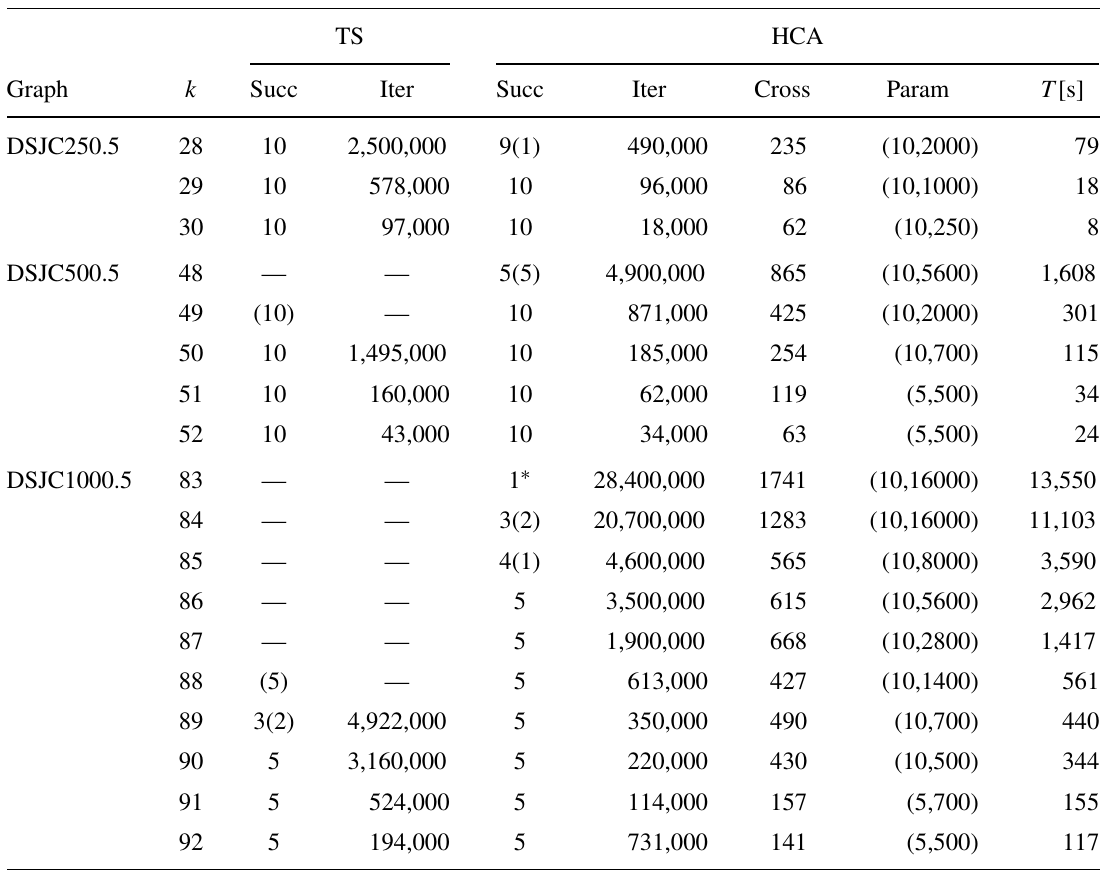
\includegraphics[height=210px]{results1.png}}
\begin{itemize}
\item HCA finds smaller k than TS, HCA is faster than TS
\end{itemize}
\end{frame}


\begin{frame}
\frametitle{Comparison with the best known results}
\centering{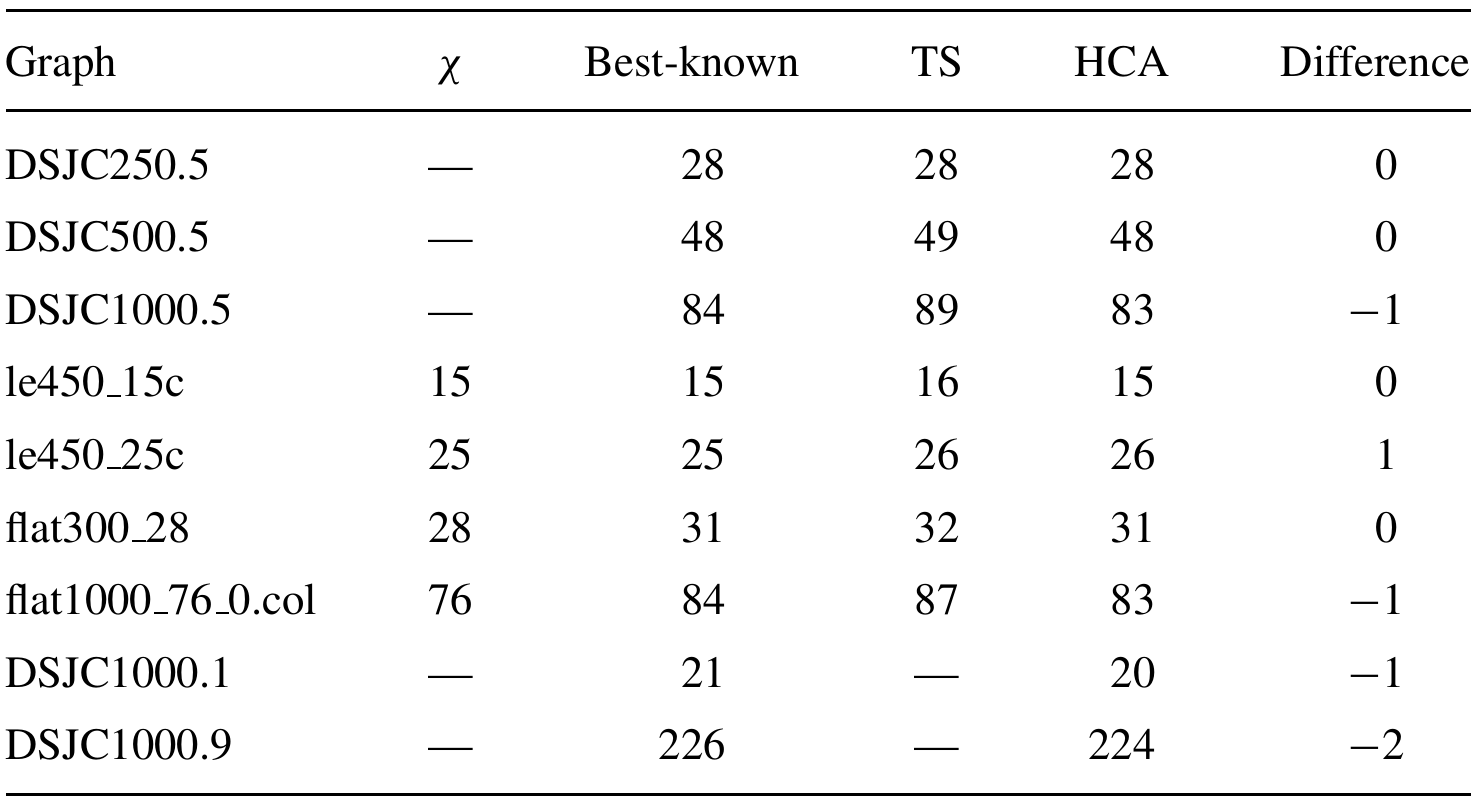
\includegraphics[height=150px]{results2.png}}
\begin{itemize}
\item HCA finds the best known result for each graph except one
\item HCA improves on the best known results for four large graphs
\end{itemize}
\end{frame}

%%%%%%%%%%%%%%%%%%%%%%%%%%%%%%%%%%%%%%%%%%%%%%%%%%%%%% Experiments and results - Prugel

\begin{frame}
\frametitle{HCA without Tabu Search}
\begin{itemize}
\item \textbf{Vertex Descent algorithm:} each vertex is taken in turn and a color selected for that vertex which gives the lowest number of conflicts
\item \textbf{A large population} eliminates the difficulties of premature convergence
\item \textbf{Generational} GA
\end{itemize}
\end{frame}

\begin{frame}
\frametitle{Experimental results}
\centering{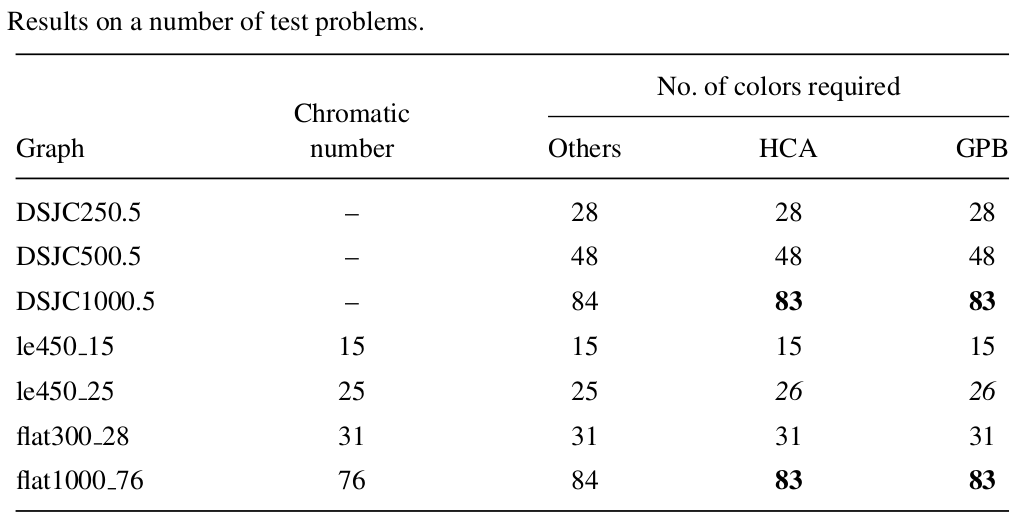
\includegraphics[height=150px]{prugel1.png}}
\begin{itemize}
\item Equally good results
\end{itemize}
\end{frame}

\begin{frame}
\begin{itemize}
\item \textit{\tiny HCA without Tabu Search:}\\
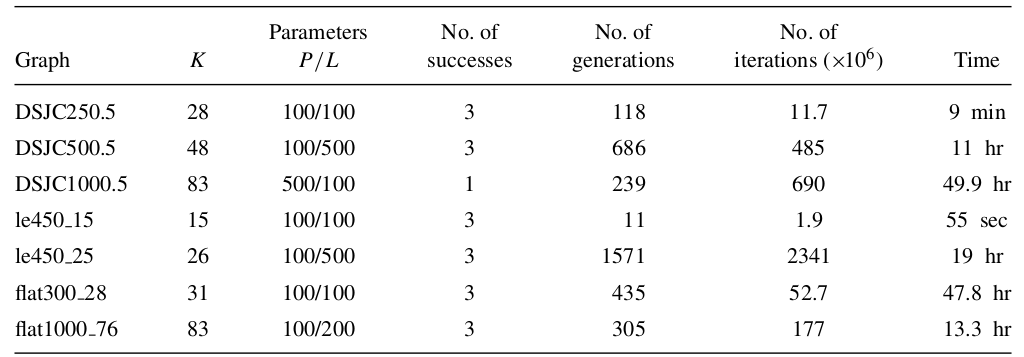
\includegraphics[height=90px]{prugel2.png}
\item \textit{\tiny HCA with Tabu Search:}\\
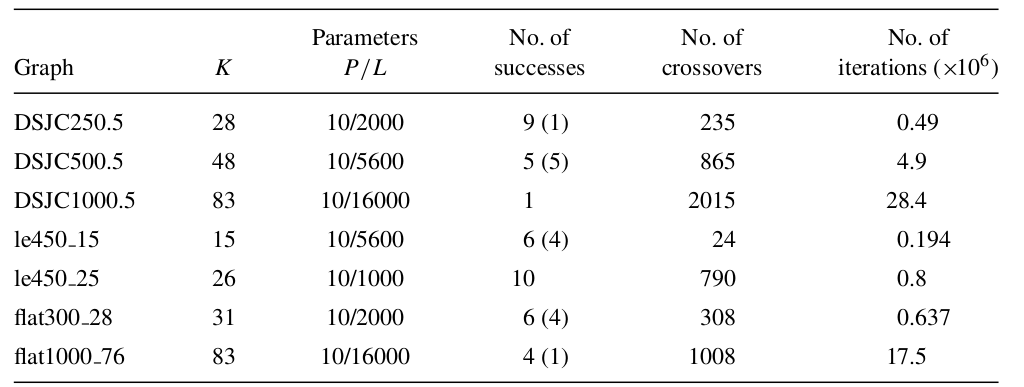
\includegraphics[height=90px]{prugel3.png}
\item More iterations between crossovers and a larger number of crossovers without Tabu Search
\end{itemize}
\end{frame}

\begin{frame}
\frametitle{Conclusions}
%Not completed
\begin{itemize}
\item A domain specific crossover operator is necessary
\item GPX is the first meaningful crossover operator for the Graph Coloring Problem
\item Longer local search is necessary for difficult problems
\item GCA component of the hybrid algorithm does not require Tabu Search
\item Tabu Search considerably reduces the number of local search iterations
\item The GPX crossover operator overcomes the permutation symmetry problem
\item The algorithm can be adapted for the Frequency Assignment Problem and Restricted Graph Coloring Problem
\end{itemize}
\end{frame} 

\end{document}
